\subsection{Projektrealisierung}
\label{sec:Projektrealisierung}

Aufbauend auf der Festlegung der Projektphasen kann das Projekt iterativ anhand der aufgezeigten Organisation
realisiert werden. An dieser Stelle setzt die konkrete Beschreibung der Realisierung des
Projektes in \citet{modelierungUndBetrieb2014} an.
Ein Einblick in diese Realisierung wäre an dieser Stelle zu umfassend und zu komplex. Aus diesem Grund werden an dieser
Stelle nur die Ergebnisse der Projektrealisierung vorgestellt.

Realisiert werden sollte eine visuelle Ansicht des neuen Campus Lingen, in dem sich der Benutzer im Stile von Google
Street View frei umsehen kann. Diese Realisierung ist gelungen und das Ergebnis ist in \abbildung{FrontendFinal}
zu sehen.

\clearpage
\begin{figure}[htb] 
\centering
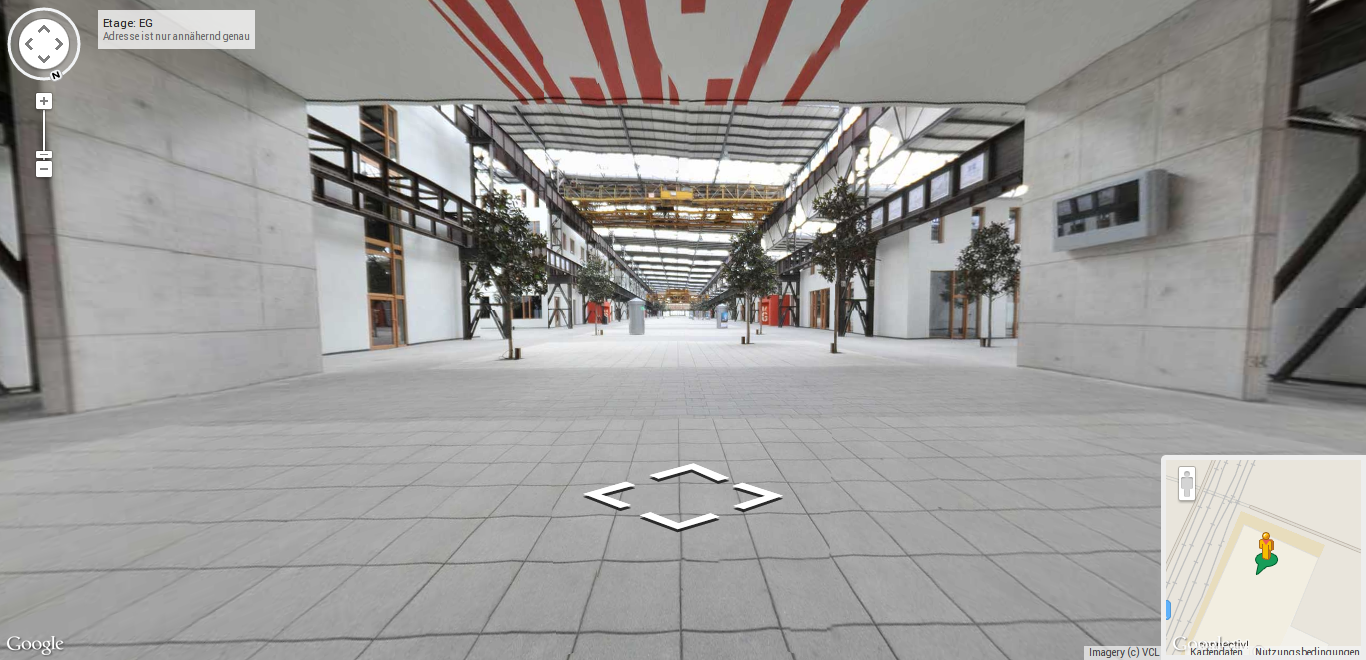
\includegraphics[width=1.0\textwidth]{FrontendFinal.png}
\caption[Abbildung der Benutzeransicht]{Ein Bildschirmfoto der fertigen Benutzeransicht\protect}
\label{fig:FrontendFinal}
\end{figure}

Neben dieser Benutzeransicht sollte darüber hinaus vor allem die Nachhaltigkeit des Projektes gewahrt werden.
Hierzu sollte ein Administrationsbereich entwickelt werden, in dem es möglich ist alle Informationen
der Benutzeransicht zu pflegen. Ein Ausschnit dieses Administrationsbereiches ist 
in \abbildung{BackendFinal} dargestellt.

\begin{figure}[htb] 
\centering
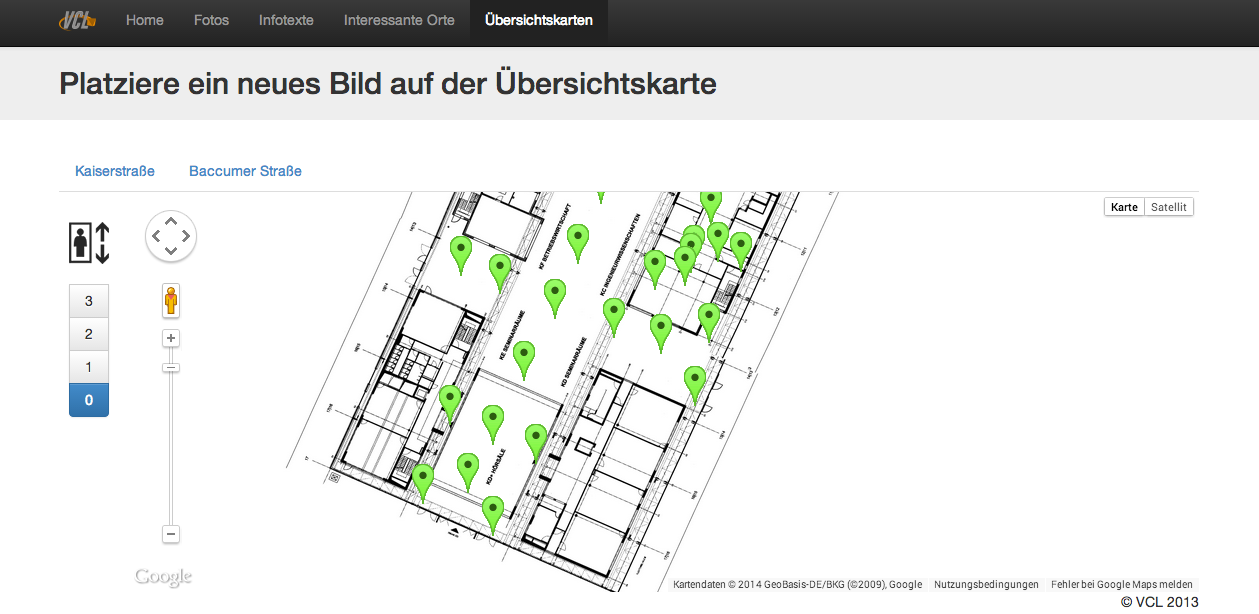
\includegraphics[width=1.0\textwidth]{BackendFinal.png}
\caption[Ausschnitt des Administrationsbereiches]{Verwalten und Platzieren von Panoramafotos im Administrationsbereich\protect}
\label{fig:BackendFinal}
\end{figure}
\clearpage